\section{Deep Learning in Planetary Science}
\label{sec:ml_planetary}
Historically, the analysis of planetary data has been driven by expert interpretation.
Geologists and geophysicists manually inspect images, optical and hyperspectral images, and radargrams to identify features of interest.
However, in the last decade, the availability of large-scale orbital datasets (e.g., HiRISE, CTX, CRISM, SHARAD, MARSIS) and advances in DL have led to a progressive shift towards automated methods based on convolutional and transformer-based architectures~\cite{Ronneberger_2015,He_2016}.

One of the earliest and most successful applications of DL in planetary science is automated crater detection and crater counting on Mars and the Moon~\cite{Silburt2019,LunarCraterDLReview}.
Impact craters are fundamental chronometers for planetary surfaces, and CNN-based detectors have been trained to identify and classify craters on Mars~\cite{Silburt2019,DeepMarsGithub} and the Moon~\cite{LunarCraterDL,LunarCraterDLReview}, achieving human-level performance with orders-of-magnitude higher throughput than manual surveys.
Architectures derived from U-Net and Fully Convolutional Networks (FCNs) are now standard for segmenting geomorphological features such as dunes, channels, and volcanic flows~\cite{Fernandez2019DuneMapping,DeepDuneMapping} from high-resolution optical imagery (e.g., HiRISE, CTX), often coupled with residual backbones such as ResNet~\cite{He_2016}.

Beyond surface morphology, DL has been applied to a wide range of planetary and terrestrial remote sensing tasks, including:
\begin{itemize}
    \item \textbf{Feature detection vs. semantic segmentation of surface units:} DL models support both object-level detection of discrete features (e.g., impact craters, boulders) and full semantic segmentation of surface units (e.g., lava flows, sedimentary deposits, polar layered terrains) from multispectral and hyperspectral images~\cite{Silburt2019,Fernandez2019DuneMapping,Wang2019DeepMars}. In the former, detectors or instance-segmentation networks localize individual features, while in the latter encoder–decoder architectures learn to assign a geological class to each pixel, producing dense surface morphology maps.
    \item \textbf{Change detection} between multi-temporal observations, used to identify active processes such as dust storms, frost deposition, or landslides by comparing deep feature representations across time~\cite{Parajuli2020DustDL,FrontiersSandstorm_2022}.
    \item \textbf{Super-resolution and enhancement} of orbital imagery, where SRGAN-like models synthesize high-resolution views from lower-resolution sensors, improving the visibility of small-scale structures of interest~\cite{Ledig2017SRGAN,Li2022SRGANRemoteSensing}. 
\end{itemize}

These developments are directly relevant for this thesis because they illustrate how DL can (i) learn robust feature representations from complex, noisy planetary data and (ii) support downstream scientific tasks such as mapping, detection, and anomaly discovery~\cite{yebasse2025advances}.
In particular, the success of encoder–decoder architectures and generative models in optical and SAR remote sensing motivates their adaptation to RS radargrams, which share many of the challenges discussed in Section~\ref{sec:rs_challenges} (e.g., speckle noise, depth-dependent attenuation, surface clutter, and the strong anisotropy between range and along-track directions), despite being physically different from natural images~\cite{yebasse2025advances}.

\begin{figure}[t]
    \centering
    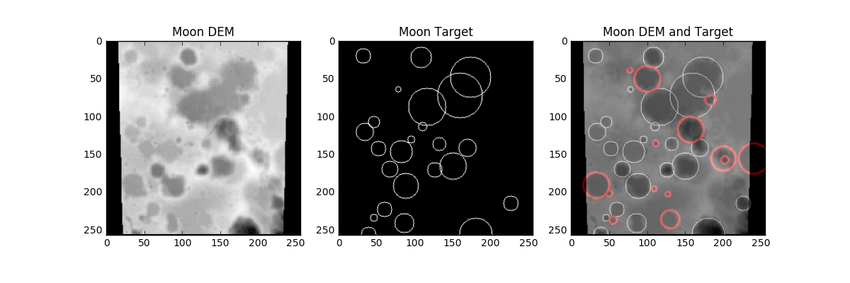
\includegraphics[width=0.75\textwidth]{images/dl_crater_segmentation}
    \caption{Example of DL-based crater detection and segmentation on planetary imagery. Convolutional encoder–decoder architectures, derived from U-Net, are widely used to detect and delineate impact craters, enabling large-scale, automated chronologic analysis. Reproduced from~\cite{Silburt2019}.}
    \label{fig:dl_crater_segmentation}
\end{figure}

\begin{figure}[t]
    \centering
    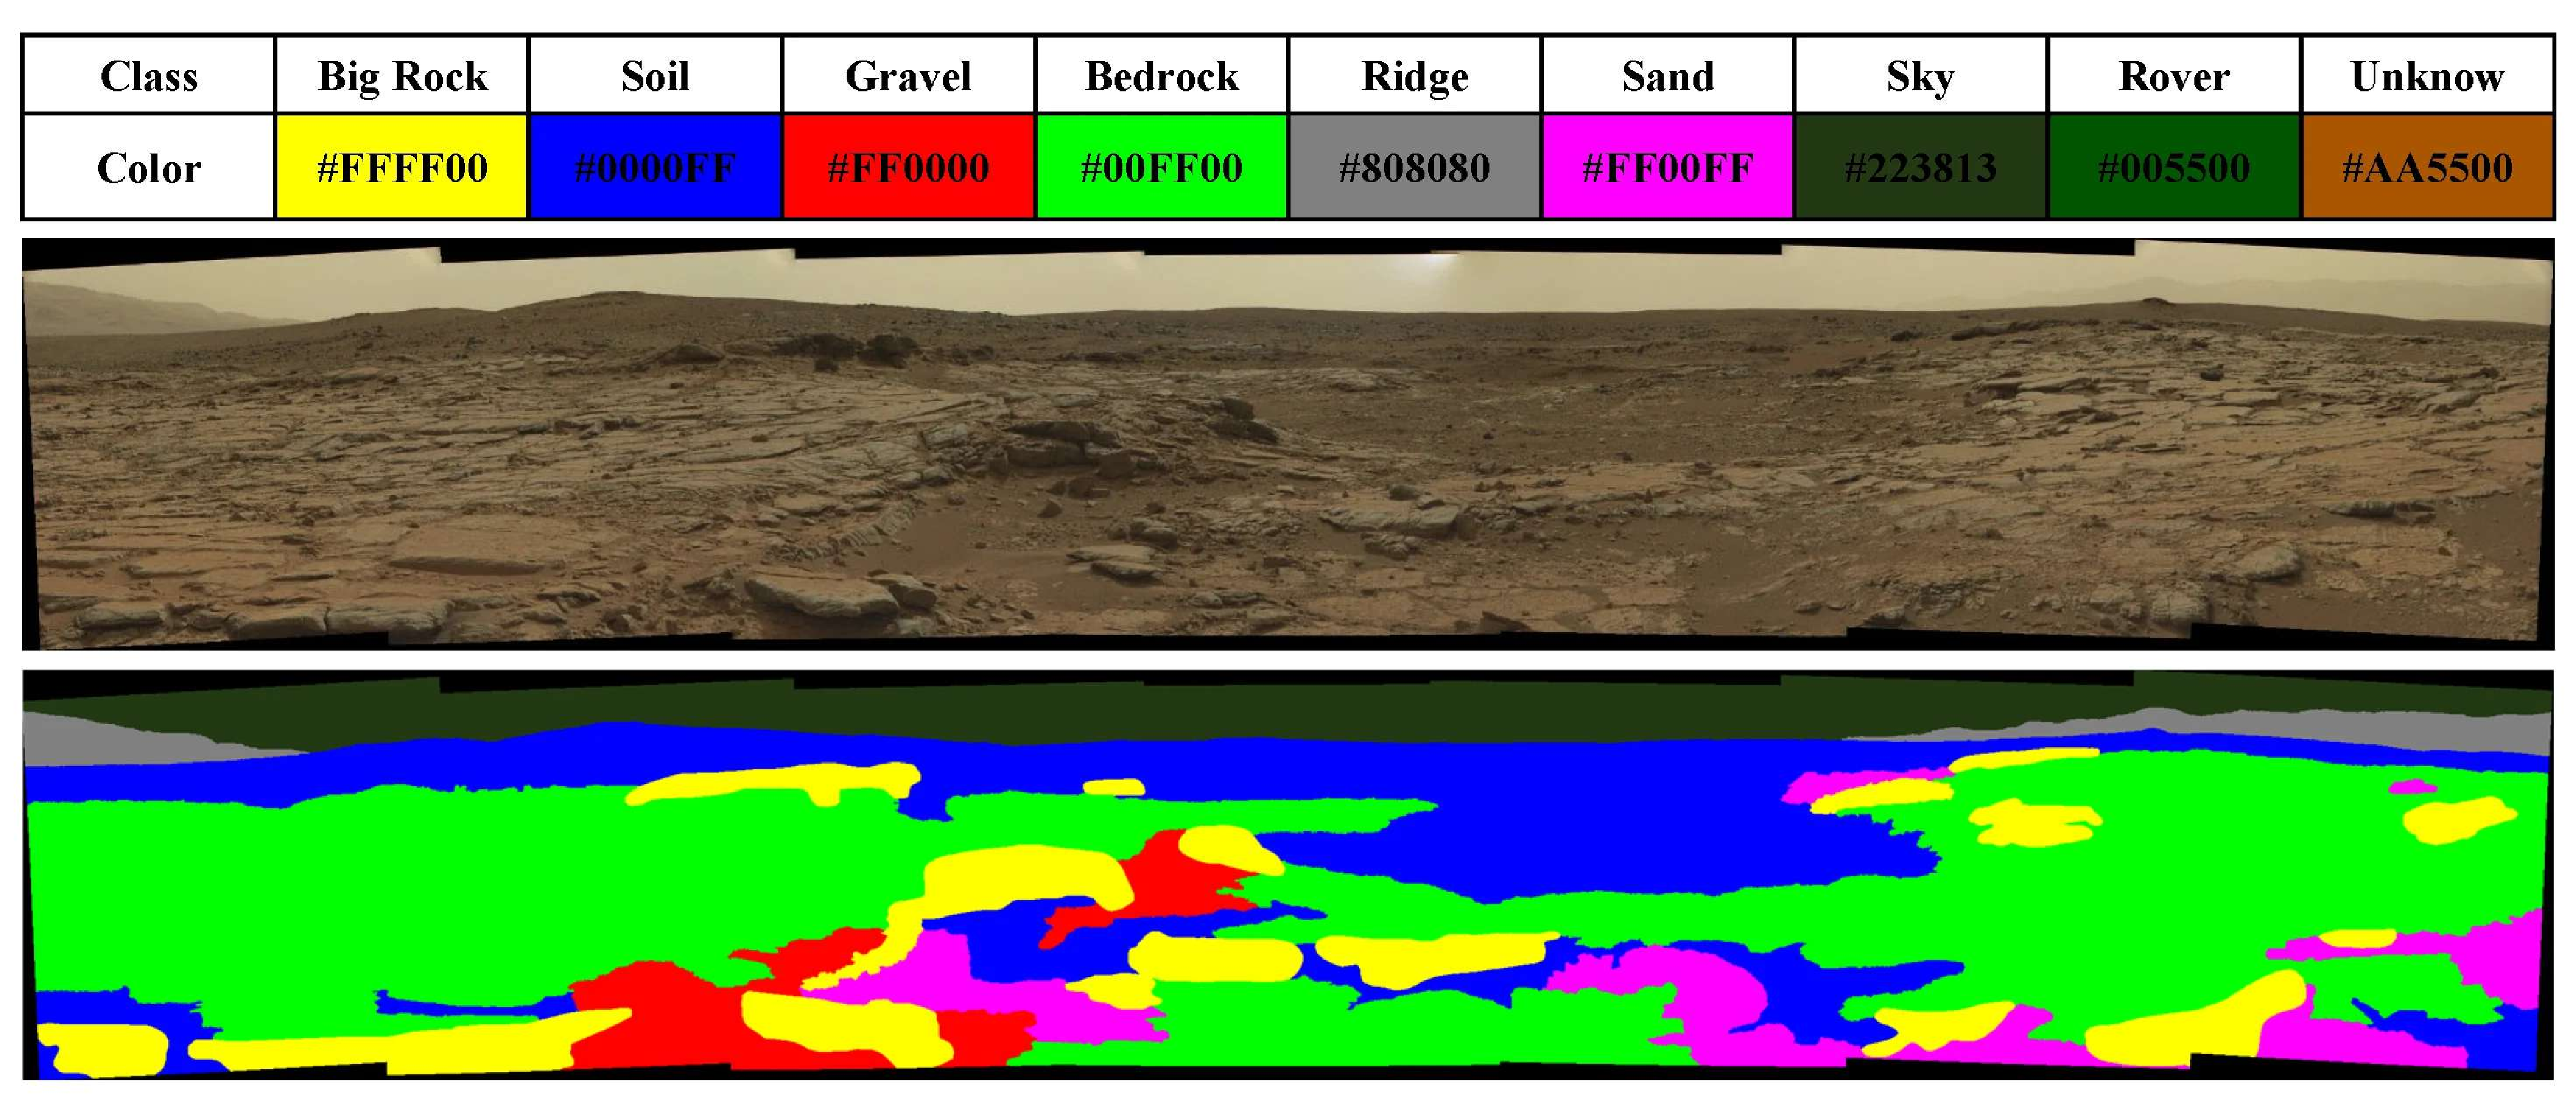
\includegraphics[width=0.85\textwidth]{images/dl_geomorph_mapping}
    \caption{Schematic illustration of DL-based geomorphological mapping from high-resolution orbital images. Semantic segmentation networks assign each pixel to a geomorphic class (e.g., lava flows, dunes, layered deposits), producing dense maps that support quantitative planetary surface studies. Example of terrain semantic segmentation reproduced from \cite{zhang2024s5mars}.}
    \label{fig:dl_geomorph_mapping}
\end{figure}

